\documentclass[serif,mathserif]{beamer}
\usepackage{etex}
\usepackage{amsmath, amsfonts, epsfig, xspace}
\usepackage{algorithm,algorithmic}
\usepackage{pstricks,pst-node}
\usepackage{multimedia}
\usepackage[normal,tight,center]{subfigure}
\setlength{\subfigcapskip}{-.5em}
\usepackage{beamerthemesplit}
\usetheme{lankton-keynote}
\usepackage{color}
\usepackage{graphicx,color}
% remove caption of figure
\usepackage[labelformat=empty]{caption}

\usepackage[none]{hyphenat} % hyphenation is ugly in slides
\usepackage{parskip}

\usepackage{relsize} % \smaller to change size

\usepackage{tikz}
\usetikzlibrary{calc}

\usetikzlibrary{arrows}

\newcommand{\TikzDraw}[2][]{
  \begin{tikzpicture}[overlay, remember picture, shift={(current page.center)}, #1]
    #2
  \end{tikzpicture}
}

\newcommand{\gridlines}{
  \TikzDraw{
    \draw[help lines,xstep=.2,ystep=.2,red!20] (current page.south west) grid (current page.north east);
    \draw[help lines,xstep=1,ystep=1,red] (current page.south west) grid (current page.north east);
    \foreach \x in {-15,-14,...,15} {
      \node [anchor=north, red] at (\x,0) {\tiny \x};
      \node [anchor=east,red] at (0,\x) {\tiny \x};
    }
  }
}

\newcommand{\DrawOnImg}[3][]
{
  \begin{tikzpicture}
    \node[anchor=south west,inner sep=0] (image) at (0,0){
      #2
    };
    \begin{scope}[x={(image.south east)},y={(image.north west)}]
      \ifthenelse{\equal{#1}{grid}}
                 {\draw[color=blue, style=dashed] (0,0) grid[xstep=.1, ystep=.1] (1.0001,1.0001);}
                 {}
                 #3
    \end{scope}
  \end{tikzpicture}
}


\author[Jiong Chen]{Jiong Chen}

\title[\hspace{2em}\insertframenumber/\inserttotalframenumber]{Stable Constrained Dynamics}

\date{September 30, 2015} %leave out for today's date to be insterted

% \institute{Zhejiang University}

\newcommand{\BOLD}[1]{\mathbf{#1}}
\newcommand{\PDIF}[2]{\frac{\partial #1}{\partial #2}}

\definecolor{DARK}{RGB}{45, 33, 73}
\definecolor{LIGHT}{RGB}{119, 52, 106}
\definecolor{TEXTLIGHT}{RGB}{213, 207, 229}
\definecolor{TEXTDARK}{RGB}{66, 66, 66}
\definecolor{BULLET}{RGB}{179, 17, 102}
\definecolor{EM}{RGB}{179,17,102}

\begin{document}

\maketitle

\begin{frame}
 \frametitle{Introduction to Time Integration}
 \begin{itemize}
  \item Explicit Euler
    \begin{eqnarray*}
     \BOLD{v}_+ &=& \BOLD{v} + h\BOLD{a} \\
     \BOLD{x}_+ &=& \BOLD{x} + h\BOLD{v}
    \end{eqnarray*}
  \item Symplectic Euler
   \begin{eqnarray*}
     \BOLD{v}_+ &=& \BOLD{v} + h\BOLD{a} \\
     \BOLD{x}_+ &=& \BOLD{x} + h\BOLD{v}_+
    \end{eqnarray*}
  \item Implicit Euler
    \begin{eqnarray*}
     \BOLD{v}_+ &=& \BOLD{v} + h\BOLD{a}_+ \\
     \BOLD{x}_+ &=& \BOLD{x} + h\BOLD{v}_+
    \end{eqnarray*}
 \end{itemize}
 \pause
 \TikzDraw {
    \node [fill=DARK!50, draw=black!50, rounded corners=3mm, text opacity=1, fill opacity=0.7] at (0.3, -2.8) {\huge \color{yellow}$(\BOLD{M}-h^2\BOLD{K})\BOLD{v}_+=\BOLD{p}+h\BOLD{f}$};
    \pause
    \draw[red, very thick] (-3.4,-3.4) -- (-3.4,-2.2) -- (0.2,-2.2) -- (0.2,-3.4) -- (-3.4,-3.4);
    \node at (-1.6, -3.7) {\color{green!50} augmented inertia};
    \draw[red, very thick] (1.8, -2.2) -- (1.8, -3.4) -- (2.4, -3.4) -- (2.4, -2.2) -- (1.8, -2.2);
    \node at (2.1, -1.8) { \color{green!50} current momentum};
    \draw[red, very thick] (3.2, -2.2) -- (3.2, -3.4) -- (4, -3.4) -- (4, -2.2) -- (3.2, -2.2);
    \node at (4.2, -3.7) { \color{green!50} external impulse};
 }
 %\gridlines
\end{frame}

\begin{frame}
 \frametitle{Hard Constraints}
 \begin{itemize}
  \item E.g. model thin inextensible objects 
  \begin{figure}
    \centering 
    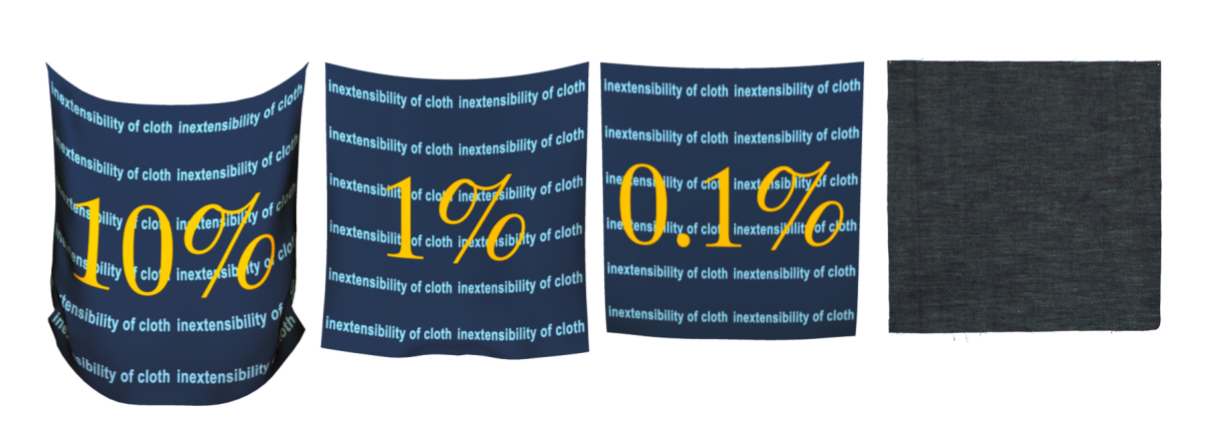
\includegraphics[scale=0.2]{img/inextensible.png}
  \end{figure}
  \item Lagrange function
    \begin{equation*}
      \mathcal{L}(t, \BOLD{x}, \BOLD{\dot x}, \BOLD{\lambda}) = \frac{1}{2}\BOLD{\dot x^T M \dot x} - V(\BOLD{x}) - \sum_i \lambda_i \phi(\BOLD{x})
    \end{equation*}
 \end{itemize}
 %\gridlines 
\end{frame}

\begin{frame}
 \frametitle{Hard Constraints}
 \begin{itemize}
    \item Euler-Lagrange equation
    \begin{equation*}
      \PDIF{\mathcal{L}}{\BOLD{x}}-\frac{d}{dt}\PDIF{\mathcal{L}}{\BOLD{\dot x}} = 0
      \Longrightarrow \BOLD{M\ddot x} = -\PDIF{V}{\BOLD{x}}-\BOLD{J^T\lambda}
    \end{equation*}
    \pause
    \TikzDraw {
      \visible<2> {
	\draw[red, very thick] (2.2, 1.2) circle (0.6cm);
	\draw[red, very thick] (3.6, 1.2) circle (0.6cm);
	\node at (2, 0.2) { \color{green!50} elastic force};
	\node at (4, 2.2) { \color{green!50} constraint force};
      }
    }
    \pause
    \item Linearization 
    \begin{equation*}
      \begin{pmatrix}
	\BOLD{M}-h^2\BOLD{K} & -\BOLD{J}^T \\
	\BOLD{J} & 0
      \end{pmatrix}
      \begin{pmatrix}
       \BOLD{v}_{+} \\ \BOLD{\mu}_{+}
      \end{pmatrix}
      =
      \begin{pmatrix}
       \BOLD{0} \\ \BOLD{0}
      \end{pmatrix}
    \end{equation*}
    \pause
 \end{itemize}
 \gridlines 
\end{frame}


%\begin{frame}
% \frametitle{Conclusion}
% \TikzDraw {
%   \visible<1-> { \node at (-1,1) 
%     {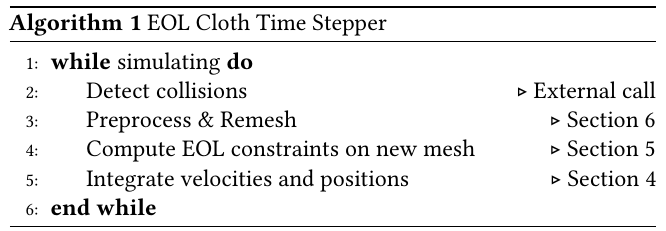
\includegraphics[scale=0.2]{pic/algorithm.png}}; 
%   }
%   \visible<1> {\node at (2,-2) 
%     {\parbox[t]{\textwidth}{\Large$\pi(x_1) = \pi(x_2) = x$}}; 
%   }
%   \visible<1> {\node at (7, -3) 
%     {\parbox[t]{\textwidth}{$\alpha\circ \tau = -\alpha\\ cos(\alpha)=cos(-\alpha)$}};
%   }
% }
% \gridlines
%\end{frame}

\begin{frame} 
  \TikzDraw {
    \node at (0, 0.5) {\Huge{Thanks!}};
  }
  %\gridlines
\end{frame}


\end{document}
